\section{Front-end}

	\subsection{Descrizione packages e classi}

	\subsubsection{SWEDesigner::Client}
\begin{figure}
			\centering
			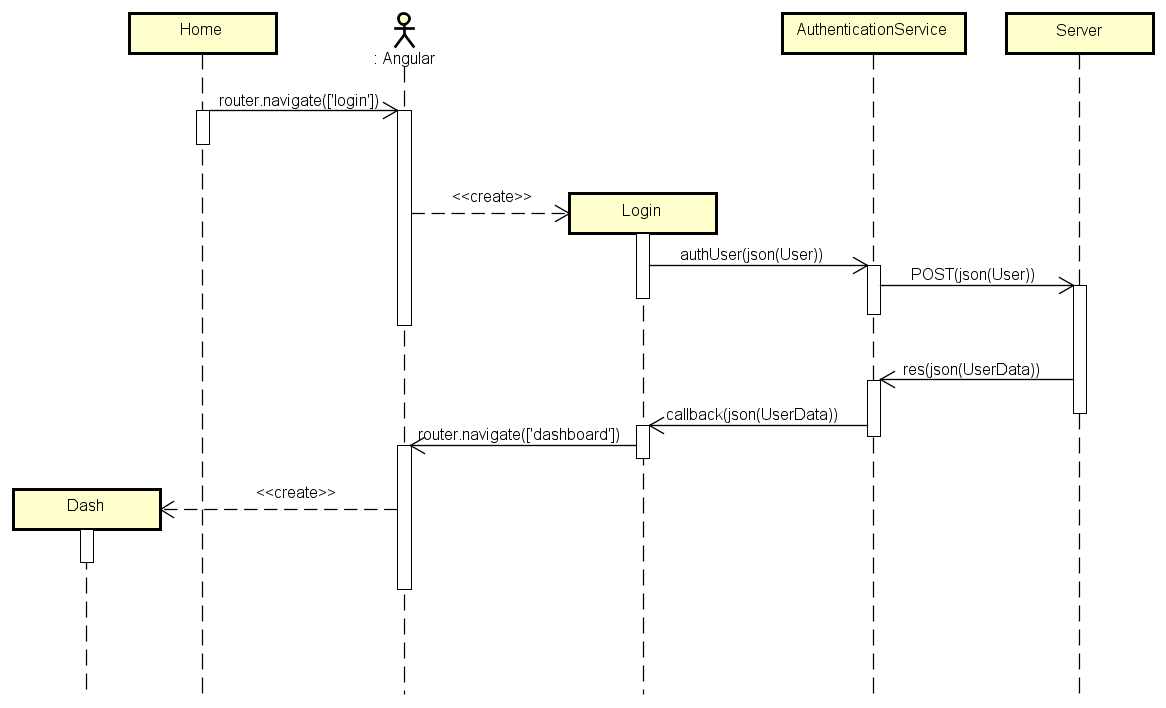
\includegraphics[scale=0.4]{Disegnetti/SequenceDiagram.png}
			\caption{Esempio di funzionamento dell'applicazione lato client}
		\end{figure}		
		\begin{figure}[h!]
			\centering
			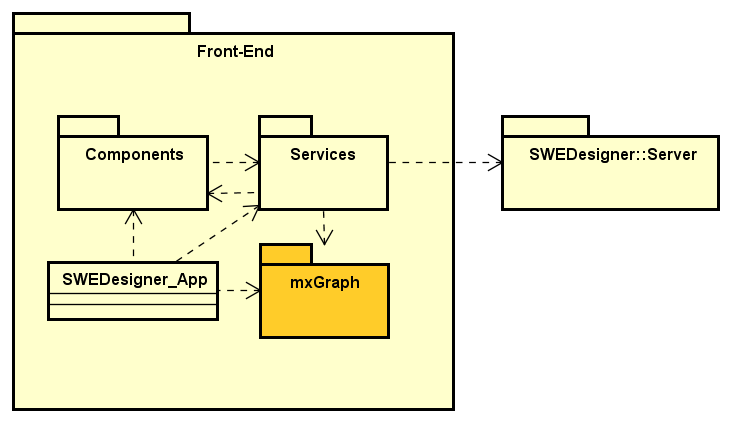
\includegraphics[scale=0.8]{Disegnetti/Front-End.png}
			\caption{Diagramma dei packages SWEDesigner::Client}
 		\end{figure}
		

		\paragraph{Informazioni sul Package}
		\begin{itemize}
			\item \textbf{Descrizione: }\\
			Package che racchiude tutta la componente di Front-end scritta in TypeScript.
			\item \textbf{Padre: }\\ SWEDesigner
			\item \textbf{Package contenuti: }
			\begin{itemize}
				\item SWEDesigner::Client::Components;
				\item SWEDesigner::Client::Services;
				\item SWEDesigner::Server;
			\end{itemize}
		\end{itemize}

		\subsubsection{SWEDesigner::Client::Components}
		 \begin{figure}[h!]
		\centering
		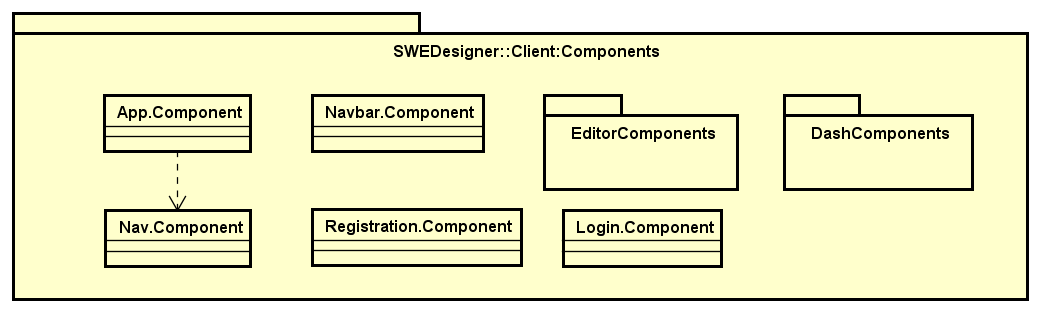
\includegraphics[scale=0.8]{Disegnetti/SWEDesigner__Client_Components.png}
		\caption{Diagramma dei packages SWEDesigner::Client::Components}
 		\end{figure}
		\paragraph{Informazioni sul Package}
		\begin{itemize}
			\item \textbf{Descrizione: }\\
			Questo package contiene tutti i components dell'applicazione
			\item \textbf{Padre: }\\ SWEDesigner::Client
			\item \textbf{Package contenuti: }
			\begin{itemize}
				\item SWEDesigner::Client::Components::Editor;
				\item SWEDesigner::Client::Components::Menu;
				\item SWEDesigner::Client::Components::ActivityFrame;
			\end{itemize}
		\end{itemize}

		\paragraph{Informazioni sulle Classi}
		\begin{itemize}
			\item SWEDesigner::Client::Components::AppComponent
			\begin{itemize}
				\item \textbf{Descrizione: }\\
				Il component descrive un contenitore per la barra di navigazione e le altre
				componenti dell'applicazione le quali sono istanziate dinamicamente all'
				interno del template http;
				\item \textbf{Utilizzo: }\\
				AppComponent è il primo component che viene istanziato tramite bootsrap.
				\item \textbf{Relazioni con altre classi: }\\
				\begin{itemize}
				\item \emph{OUT} SWEDesigner::Client::Services::editorService. Utilizza i servizi per effettuare azioni all'interno dell'editor.
				\item \emph{OUT} SWEDesigner::Client::Services::menuService. Utilizza i servizi per l'applicazione delle funzionalità del menu.
				\item \emph{OUT } SWEDesigner::Client::Services::NavbarComponent. Permette la navigazione all'interno dell'applicazione
				\end{itemize}
			\end{itemize}
			\item SWEDesigner::Client::Components::NavbarComponent
			\begin{itemize}
				\item \textbf{Descrizione: }\\
				Questo component permette la navigazione all'interno dell'applicazione
				tramite links;
				\item \textbf{Utilizzo: }\\
				NavbarComponent è istanziato per bootstrap subito dopo dell'AppComponent
				\item \textbf{Relazioni con altre classi: }
				\begin{itemize}
				\item \emph{IN} SWEDesigner::Client::Component::AppComponent. Richiama il componente di navigazione.
				\end{itemize}
			\end{itemize}
			
			\item SWEDesigner::Client::Components::RegistrationComponent
			\begin{itemize}
				\item \textbf{Descrizione: }\\
				È il componente che descrive la pagina di registrazione dell'applicazione,
				mette a disposizione dell'utente un form dove iserire le informazioni
				necessarie alla creazione di un nuovo account utente. Gestisce le
				operazioni e la logica applicativa per la registrazione servendosi dei
				metodi forniti dal servizio AuthenticationService;
				\item \textbf{Utilizzo: }\\
				Questo componente viene instanziato dinamicamente dal servizio Router del
				 framework Angular qunado viene richiesta la pagina di registrazione.
				 \item \textbf{Relazioni con altre classi: }
				\begin{itemize}
				\item \emph{OUT} SWEDesigner::Client::Services::accountService. Permette le operazioni di registrazione.
				\end{itemize}
			\end{itemize}
			\item SWEDesigner::Client::Components::LoginComponent
			\begin{itemize}
				\item \textbf{Descrizione: }\\
				È il componente che descrive la pagina di login dell'applicazione,
				mette a disposizione dell'utente un form dove iserire username e password.
				Gestisce le operazioni e la logica applicativa per il login servendosi dei
				metodi forniti dal servizio AuthenticationService;
				\item \textbf{Utilizzo: }\\
				Questo componente viene instanziato dinamicamente dal servizio Router del
				framework Angular qunado viene richiesta la pagina di login.
				\item \textbf{Relazioni con altre classi: }
				\begin{itemize}
				\item \emph{OUT} SWEDesigner::Client::Services::accountService. Permette le operazioni di login.
				\end{itemize}
			\end{itemize}
		\end{itemize}

		\subsubsection{SWEDesigner::Client::Components::Editor}
		 \begin{figure}[h!]
		\centering
		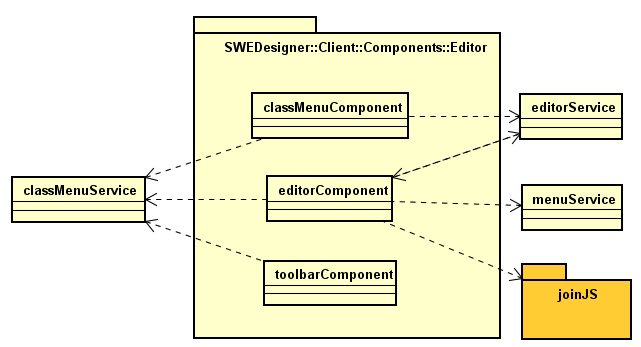
\includegraphics[scale=0.8]{Disegnetti/SWEDesigner__Client__Components__editor.png}
		\caption{Diagramma dei packages SWEDesigner::Client::Components::Editor}
 		\end{figure}
		\paragraph{Informazioni sul Package}
		\begin{itemize}
			\item \textbf{Descrizione: }\\
			Il package contiene tutte le components riguardanti l'editor dei diagrammi.
			\item \textbf{Padre: }\\ SWEDesigner::Client::Components
		\end{itemize}

		\paragraph{Informazioni sulle Classi}
		\begin{itemize}
			\item SWEDesigner::Client::Components::Editor::ToolbarComponent
			\begin{itemize}
				\item \textbf{Descrizione: }\\
				ToolbarComponent descrive il menu dal quale l'utente può selezionare gli
				strumenti per disegnare i diagrammi all'interno degli appositi frame. Si
				occupa delle operazioni e della parte logica, riguardante la costruzione
				dei diagrammi, servendosi dei metodi forniti delle API della libreria grafica;
				\item \textbf{Utilizzo: }\\
				ToolbarComponent componente viene istanziato per bootstrap dopo che è stato
				istanziato il component AppComponent.
				\item \textbf{Relazioni con altre classi: }
				\begin{itemize}
				\item \emph{OUT} SWEDesigner::Client::Services::classMenuService. Permette le operazioni di selezione dal menu degli strumenti.
				\end{itemize}
			\end{itemize}
			\item SWEDesigner::Client::Components::Editor::editorComponent
			\begin{itemize}
				\item \textbf{Descrizione: }\\
				Component che contiene la rappresentazione grafica dei diagrammi disegnati dall'utente
				\item \textbf{Utilizzo: }\\
				Questo componente viene instanziato dinamicamente dal servizio Router del
				framework Angular quando viene richiesta la pagina dell'editor diagrammi.
				\item \textbf{Relazioni con altre classi: }
				\begin{itemize}
				\item \emph{OUT} SWEDesigner::Client::Services::classMenuService. Permette le operazioni modifica dei campi di un oggetto selezionato.
				\item \emph{OUT} SWEDesigner::Client::Services::menuService. Permette l'applicazione delle funzionalità fornite dal menu.
				\item \emph{OUT} SWEDesigner::Client::Services::editorService. Permette le operazioni di iterazione con il componente classMenuComponent.
				\item \emph{IN} SWEDesigner::Client::Services::editorService. Permette le operazioni di ricezione delle informazioni che vengono elaborate dal componente classMenuComponent.
				\item \emph{OUT} jointJS. Permette l'utilizzo delle funzionalità fornite dalla libreria grafica.
				\end{itemize}
			\end{itemize}
			
			\item SWEDesigner::Client::Components::Editor::classMenuComponent
			\begin{itemize}
			\item \textbf{Descrizione: }\\
			Component che permette la modifica dei campi dati di un oggetto selezionato nell'editorComponent
			\item \textbf{Utilizzo: }\\
			Component figlio di editorComponent viene visualizzato quando viene selezionato un elemento editabile nell'editorComponent.
			\item \textbf{Relazioni con altre classi: }
			\begin{itemize}
			\item \emph{OUT} SWEDesigner::Client::Services::editorService. Permette le operazioni di comunicazione con il componente editorComponent.
			\item \emph{OUT} SWEDesigner::Client::Services::classMenuService. Permette le operazioni di iterazione con il componente editorComponent per visualizzare o meno il component.
			\end{itemize}
			\end{itemize}						
			
			\subsubsection{SWEDesigner::Client::Components::Menu}
		 \begin{figure}[h!]
		\centering
		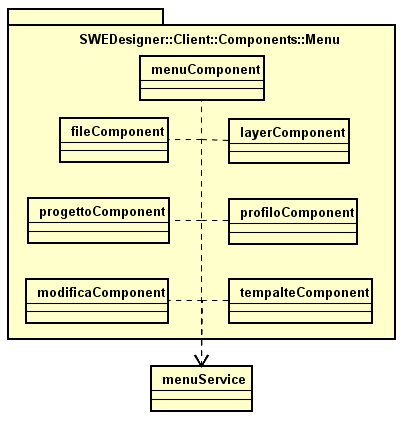
\includegraphics[scale=0.8]{Disegnetti/SWEDesigner__Client__Components__menu.png}
		\caption{Diagramma dei packages SWEDesigner::Client::Components::Menu}
 		\end{figure}
		\paragraph{Informazioni sul Package}
		\begin{itemize}
			\item \textbf{Descrizione: }\\
			Il package contiene tutti i components riguardanti la gestione delle funzionalirà fornite dal menu.
			\item \textbf{Padre: }\\ SWEDesigner::Client::Components
		\end{itemize}

		\paragraph{Informazioni sulle Classi}
		\begin{itemize}
		\item SWEDesigner::Client::Component::Menu::menuComponent		
		\begin{itemize}
			\item \textbf{Descrizione:}\\
			Component che contiene l'insieme di funzionalità fornite all'utente per la gestione dei progetti, dei propri dati personali, e della rappresentazione dei grafici su cui sta lavorando.
			\item \textbf{Utilizzo:}\\
			menuComponent viene istanziato per bootstrap dopo che è stato istanziato il component appComponent;
			\item \textbf{Relazione con altre classi:}\\
			\begin{itemize}
			\item \emph{OUT} SWEDesigner::Client::Services::menuService.
			\end{itemize}
		\end{itemize}
		
		\item SWEDesigner::Client::Component::Menu::fileComponent		
		\begin{itemize}
			\item \textbf{Descrizione:}\\
			Component che contiene l'insieme di funzionalità fornite all'utente per la gestione del progetto attualmente in uso.
			\item \textbf{Utilizzo:}\\
			fileComponent viene istanziato per bootstrap dopo che è stato istanziato il component menuComponent;
			\item \textbf{Relazione con altre classi:}\\
			\begin{itemize}
			\item \emph{OUT} SWEDesigner::Client::Services::menuService. Permette le operazioni di salvataggio ed esportazione del progetto in uso.
			\end{itemize}
		\end{itemize}
		
		\item SWEDesigner::Client::Component::Menu::layerComponent		
		\begin{itemize}
			\item \textbf{Descrizione:}\\
			Component che contiene l'insieme di funzionalità fornite all'utente per la gestione dei layer del progetto in uso.
			\item \textbf{Utilizzo:}\\
			layerComponent viene istanziato per bootstrap dopo che è stato istanziato il component menuComponent;
			\item \textbf{Relazione con altre classi:}\\
			\begin{itemize}
			\item \emph{OUT} SWEDesigner::Client::Services::menuService. Permette le operazioni di gestione dei layer del progetto in uso.
			\end{itemize}
		\end{itemize}
		
		\item SWEDesigner::Client::Component::Menu::progettoComponent		
		\begin{itemize}
			\item \textbf{Descrizione:}\\
			Component che contiene l'insieme di funzionalità fornite all'utente per la gestione dei propri progetti salvati
			\item \textbf{Utilizzo:}\\
			progettoComponent viene istanziato per bootstrap dopo che è stato istanziato il component menuComponent;
			\item \textbf{Relazione con altre classi:}\\
			\begin{itemize}
			\item \emph{OUT} SWEDesigner::Client::Services::menuService. Permette le operazioni di gestione dei propri progetti.
			\end{itemize}
		\end{itemize}
		
		\item SWEDesigner::Client::Component::Menu::profiloComponent		
		\begin{itemize}
			\item \textbf{Descrizione:}\\
			Component che contiene l'insieme di funzionalità fornite all'utente per la gestione dei propri dati personali.
			\item \textbf{Utilizzo:}\\
			profiloComponent viene istanziato per bootstrap dopo che è stato istanziato il component menuComponent;
			\item \textbf{Relazione con altre classi:}\\
			\begin{itemize}
			\item \emph{OUT} SWEDesigner::Client::Services::menuService. Permette le operazioni di gestione dei propri dati personali.
			\end{itemize}
		\end{itemize}
		
		\item SWEDesigner::Client::Component::Menu::modificaComponent		
		\begin{itemize}
			\item \textbf{Descrizione:}\\
			Component che contiene l'insieme di funzionalità fornite all'utente per la modifica del progetto in uso, come ad esempio effettuare lo zoom, oppre eliminare o copiare un elemento selezionato.
			\item \textbf{Utilizzo:}\\
			modificaComponent viene istanziato per bootstrap dopo che è stato istanziato il component menuComponent;
			\item \textbf{Relazione con altre classi:}\\
			\begin{itemize}
			\item \emph{OUT} SWEDesigner::Client::Services::menuService. Permette le operazioni di modifica sugli elementi del progetto in uso.
			\end{itemize}
		\end{itemize}
		
\item SWEDesigner::Client::Component::Menu::templateomponent		
		\begin{itemize}
			\item \textbf{Descrizione:}\\
			Component che contiene l'insieme di funzionalità fornite all'utente per l'importazione e gestione dei template.
			\item \textbf{Utilizzo:}\\
			templateComponent viene istanziato per bootstrap dopo che è stato istanziato il component menuComponent;
			\item \textbf{Relazione con altre classi:}\\
			\begin{itemize}
			\item \emph{OUT} SWEDesigner::Client::Services::menuService. Permette le operazioni di gestione ed importazione dei template.
			\end{itemize}
		\end{itemize}		
		\end{itemize}	
		

\subsubsection{SWEDesigner::Client::Components::ActivityFrame}
		 
		\paragraph{Informazioni sul Package}
		\begin{itemize}
			\item \textbf{Descrizione: }\\
			Il package contiene i components riguardanti la gestione dell'activity frame, per la visione del flusso del programma.
			\item \textbf{Padre: }\\ SWEDesigner::Client::Components
		\end{itemize}

		\paragraph{Informazioni sulle Classi}
		\begin{itemize}				
		\item SWEDesigner::Client::Components::ActivityFrame::activityFrameComponent
			\begin{itemize}
				\item \textbf{Descrizione: }\\
				Component che descrive la struttura del frame dove l'utente può visualizzare
				l'activity frame che rappresenta il flusso logico del programma.
				\item \textbf{Utilizzo: }\\
				Questo component viene istanziato per bootstrap dopo l'istanziazione
				del component AppComponent.
				\item \textbf{Relazioni con altre classi: }
				\begin{itemize}
				\item \emph{OUT} SWEDesigner::Client::Services::activityFrameService. Permette le operazioni navigazione dell'activity frame.
			\end{itemize}
			\end{itemize}
			
		\end{itemize}
		
		

			
%			\item SWEDesigner::Client::Components::Editor::MenuComponent
%			\begin{itemize}
%				\item \textbf{Descrizione: }\\
%				Component che descrive il menu dell'edito dei diagrammi. Il menu da la
%				possibilità all'utente di salvare, esportare, compilare o uscire dal progetto
%				visualizzato nell'editor dei diagrammi. Si occupa delle operazioni e della
%				logica applicativa per le operazioni, precedentemente elencate, servendosi
%				dei metodi messi a disposizione dai servizi contenuti nel package
%				ProjectServices;
%				\item \textbf{Utilizzo: }\\
%				MenuComponent componente viene istanziato per bootstrap dopo che è stato
%				istanziato il component EditorComponent.
%			\end{itemize}
%			\item SWEDesigner::Client::Components::EditorComponents::MethodComponent
%			\begin{itemize}
%				\item \textbf{Descrizione: }\\
%				MethodComponent descrive il frame dove l'utente può disegnare gli activity
%				diagrams per definire i metodi di una classe disegnata nel frame del
%				diagramma delle classi. Si occupa delle operazioni e logica applicativa per
%				la generazione dei diagrammi dei metodi, par fare questo si serve dell'API
%				della libreria grafica;
%				\item \textbf{Utilizzo: }\\
%				Questo component viene istaziato per bootstrap dopo l'istanziazione del
%				componente ClassFrameComponent.
%			\end{itemize}
%			
%			\item SWEDesigner::Client::Components::EditorComponents::ClassFrameComponent
%			\begin{itemize}
%				\item \textbf{Descrizione: }\\
%				ClassFrameComponent descrive la struttura del frame dove l'utente può
%				generare, modificare e cancellare le classi che compongono il suo progetto.
%				Si occupa delle operazioni che portano alla corretta visualizzazione del diagramma
%				servendosi dell'API della libreria grafica;
%				\item \textbf{Utilizzo: }\\
%				Questo component viene istanziato per bootstrap dopo l'istanziazione
%				del component EditorComponent.
%			\end{itemize}
%			\item SWEDesigner::Client::Components::EditorComponents::BreadcrumbComponent
%			\begin{itemize}
%				\item \textbf{Descrizione: }\\
%				Component che facilita la navigazione all'interno del ActivityFrameComponent;
%				\item \textbf{Utilizzo: }\\
%				BreadcrumbComponent component viene istanziato per bootstrap dopo l'istanziazione
%				del component ActivityFrameComponent.
%			\end{itemize}
%		\end{itemize}
%
%		\subsubsection{SWEDesigner::Client::Components::DashboardComponents}
%		 \begin{figure}[h!]
%		\centering
%		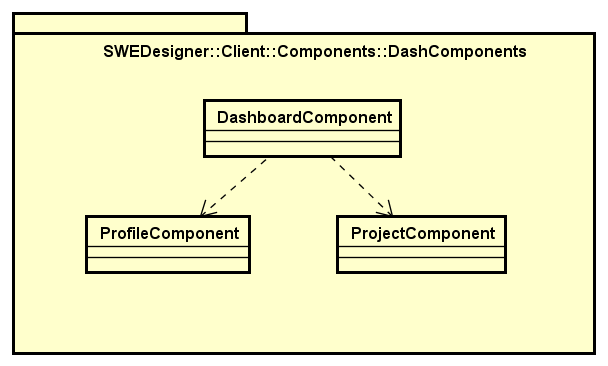
\includegraphics[scale=0.4]{Disegnetti/SWEDesigner__Client__Components__DashComponents.png}
%		\caption{Diagramma dei packages SWEDesigner::Client::Components::DashComponents}
% 		\end{figure}
%		\paragraph{Informazioni sul Package}
%		\begin{itemize}
%			\item \textbf{Descrizione: }\\
%			Il package contiene tutti i components riguardanti la gestione del profilo
%			e dei progetti dell'utente.
%			\item \textbf{Padre: }\\ SWEDesigner::Client::Components
%		\end{itemize}
%
%		\paragraph{Informazioni sulle Classi}
%		\begin{itemize}
%			\item SWEDesigner::Client::Components::DashComponents::DashComponent
%			\begin{itemize}
%				\item \textbf{Descrizione: }\\
%				Component che definisce la pagina dove l'utente è reindirizzato dopo aver
%				effettuato il login, contiene all'interno del template html gli elementi
%				per l'istanziazione del ProfileComponent e del ProjectComponent.
%				\item \textbf{Utilizzo: }\\
%				Questo componente viene instanziato dinamicamente dal servizio Router del
%				framework Angular subito dopo aver effettuato il login.
%			\end{itemize}
%			\item SWEDesigner::Client::Components::DashComponents::ProfileComponent
%			\begin{itemize}
%				\item \textbf{Descrizione: }\\
%				ProfileComponent contiene le informazioni personali dell'utente. Si occupa
%				delle operazioni che permettono il recupero dei dati utente servendosi di
%				metodi forniti dal servizio AuthenticationService.
%				\item \textbf{Utilizzo: }\\
%				Questo componenet viene istanziato per bootstrap dopo l'istanziazione
%				del component DashComponent.
%			\end{itemize}
%			\item SWEDesigner::Client::Components::DashComponents::ProjectComponent
%			\begin{itemize}
%				\item \textbf{Descrizione: }\\
%				ProfileComponent contiene la lista dei progetti salvati dall'utente, e
%				fornisce dei metodi per la modifica e la cancellazione dei progetti. Si
%				occupa delle operazioni che permettono il recupero delle informazioni sui
%				progetti servendosi di metodi forniti dal servizio ProjManagService.
%				\item \textbf{Utilizzo: }\\
%				Questo componenet viene istanziato per bootstrap dopo l'istanziazione
%				del component DashComponent.
%			\end{itemize}
%		\end{itemize}

\subsubsection{SWEDesigner::Client::Service}
		 \begin{figure}[h!]
		\centering
		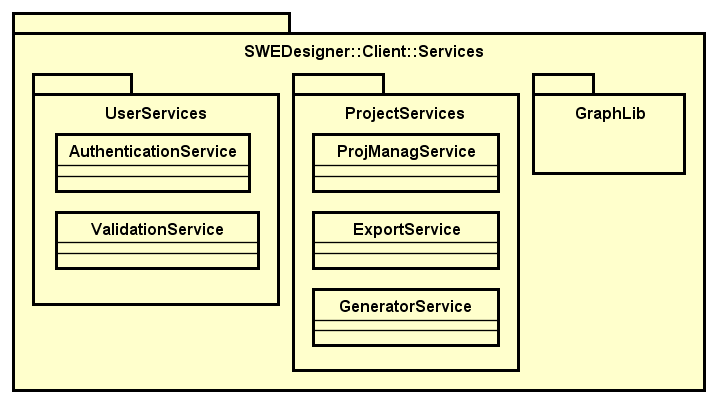
\includegraphics[scale=0.8]{Disegnetti/SWEDesigner__Client__Services.png}
		\caption{Diagramma dei packages SWEDesigner::Client::Service}
 		\end{figure}
		\paragraph{Informazioni sul Package}
		\begin{itemize}
			\item \textbf{Descrizione: }\\
<<<<<<< HEAD
			Il package contiene i servizi per le operazioni di iterazione tra i component e il server
=======
			Il package contiene i servizi per le operazioni con la libreria grafica
			\emph{jointJS} e con il server.
>>>>>>> 5b0e770cd50810b1dae7eef607dbb86704a3aec0
			\item \textbf{Padre: }\\ SWEDesigner::Client
			\item \textbf{Package contenuti: }
			\begin{itemize}
				\item SWEDesigner::Client::Services::Models;
			\end{itemize}
		\end{itemize}
		\paragraph{Informazioni sulle Classi}
		\begin{itemize}
		\item SWEDesigner::Client::Services::menuService
		\begin{itemize}
			\item \textbf{Descrizione:}\\
			Classe che definisce i metodi per le operazioni fornite all'utente dal menu;
			\item \textbf{Utilizzo:}\\
			É istaziata dal framework Angular e i suoi metodi sono utilizzati dal component menuComponent;
			\item \textbf{Relazioni con altre classi: }
			\begin{itemize}
			\item \emph{IN} SWEDesigner::Client::Components::Menu::menuComponent
			\item \emph{IN} SWEDesigner::Client::Components::Menu::fileComponent. Fornisce i metodi per il salvataggio del file in uso e la generazione del codice;
			\item \emph{IN} SWEDesigner::Client::Components::Menu::layerComponent. Fornisce i metodi per la gestione dei layer;
			\item \emph{IN} SWEDesigner::Client::Components::Menu::progettoComponent. Fornisce i metodi per la gestione dei progetti;
			\item \emph{IN} SWEDesigner::Client::Components::Menu::profiloComponent. Fornisce i metodi per la gestione del profilo utente;
			\item \emph{IN} SWEDesigner::Client::Components::Menu::modificaComponent. Fornisce i metodi per la modifica degli elementi dei diagrammi;
			\item \emph{IN} SWEDesigner::Client::Components::Menu::templateComponent. Fornisce i metodi per la gestione dei template;
			\item \emph{IN} SWEDesigner::Client::Components::Editor::editorComponent. Fornisce i metodi per effettuare operazioni all'interno dell'editor dei diagrammi.
			\end{itemize}
		\end{itemize}
		
		\item SWEDesigner::Client::Services::editorService
		\begin{itemize}
			\item \textbf{Descrizione:}\\
			Classe che definisce i metodi per le operazioni all'interno dei diagrammi e la comunicazione tra componenti e server;
			\item \textbf{Utilizzo:}\\
			É istaziata dal framework Angular e i suoi metodi sono utilizzati dai component editorComponent e classMenuComponent;
			\item \textbf{Relazioni con altre classi: }
			\begin{itemize}
			\item \emph{IN}  SWEDesigner::Client::Components::editorComponent. Fornisce i metodi per effettuare operazioni all'interno dell'editor dei diagrammi;
			\item \emph{IN}  SWEDesigner::Client::Components::classMenuComponent. Fornisce i metodi per effettuare operazioni su un elemento selezionato all'interno dell'editor dei diagrammi;
			\item \emph{IN}  SWEDesigner::Client::Services::Models::Global. Fornisce i metodi per la storicizzazione dei dati in liste;
			\end{itemize}
		\end{itemize}
		
		\item SWEDesigner::Client::Services::toolbarService
		\begin{itemize}
			\item \textbf{Descrizione:}\\
			Classe che definisce i metodi per le operazioni di inserimento di nuovi elementi all'interno dell'editor di diagrammi;
			\item \textbf{Utilizzo:}\\
			É istaziata dal framework Angular e i suoi metodi sono utilizzati dal component editorComponent;
			\item \textbf{Relazioni con altre classi: }
			\begin{itemize}
			\item \emph{IN}  SWEDesigner::Client::Components::Editod::editorComponent. Fornisce i metodi per inserire nuovi elementi all'interno dell'editor dei diagrammi;
			\end{itemize}
		\end{itemize}
		
		\item SWEDesigner::Client::Services::activityFrameService
		\begin{itemize}
			\item \textbf{Descrizione:}\\
			Classe che definisce i metodi per le operazioni di navigazione tra i metodi all'interno dell'activity frame;
			\item \textbf{Utilizzo:}\\
			É istaziata dal framework Angular e i suoi metodi sono utilizzati dal component activityFrameComponent;
			\item \textbf{Relazioni con altre classi: }
			\begin{itemize}
			\item \emph{IN}  SWEDesigner::Client::Components::ActivityFrame::activityFrameComponent. Fornisce i metodi per la navigazione tra i vari metodi all'interno dell'activity frame;
			\end{itemize}
		\end{itemize}
		
		\item SWEDesigner::Client::Services::classMenuService
		\begin{itemize}
			\item \textbf{Descrizione:}\\
			Classe che definisce i metodi per le operazioni di modifica di un elemento selezionato all'interno del diagramma rappresentato
			\item \textbf{Utilizzo:}\\
			É istaziata dal framework Angular e i suoi metodi sono utilizzati dal component classMenuService;
			\item \textbf{Relazioni con altre classi: }
			\begin{itemize}
			\item \emph{IN}  SWEDesigner::Client::Components::Editor::classMenuComponent. Fornisce i metodi per la modifica di un elemento selezionato all'interno del diagramma;
			\item \emph{IN}  SWEDesigner::Client::Components::Editor::editorComponent. Fornisce i metodi di comunicazione e di passaggio di informazioni tra editorComponent e classMenuComponent per un elemento selezionato;
			\end{itemize}
		\end{itemize}
		
		\item SWEDesigner::Client::Services::accountService
		\begin{itemize}
			\item \textbf{Descrizione:}\\
			Classe che definisce i metodi di registrazione, login e recupero dati utente dal server
			\item \textbf{Utilizzo:}\\
			É istaziata dal framework Angular e i suoi metodi sono utilizzati dai component registrationComponent e loginComponent;
			\item \textbf{Relazioni con altre classi: }
			\begin{itemize}
			\item \emph{IN}  SWEDesigner::Client::Components::registrationComponent. Fornisce i metodi per la registrazione di un nuovo utente e la comunicazione con il server;
			\item \emph{IN}  SWEDesigner::Client::Components::loginComponent. Fornisce i metodi per il login di un utente registrato e la convalida dal server.		
			\end{itemize}
		\end{itemize}
		
		\end{itemize}



\subsubsection{SWEDesigner::Client::Service::Models}
		 \begin{figure}[h!]
		\centering
		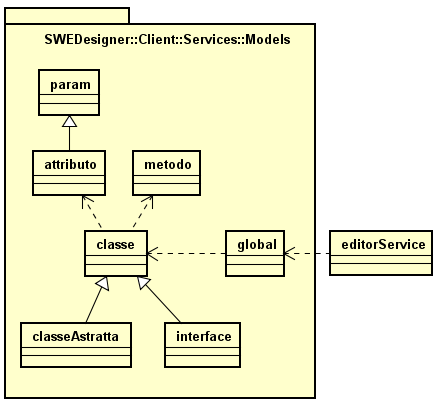
\includegraphics[scale=0.8]{Disegnetti/SWEDesigner__Client__Services__Model.png}
		\caption{Diagramma dei packages SWEDesigner::Client::Service::Models}
 		\end{figure}
		\paragraph{Informazioni sul Package}
		\begin{itemize}
			\item \textbf{Descrizione: }\\
			Il package contiene moduli necessari a storicizzare i dati inseriti all'interno dei diagrammi.
			\item \textbf{Padre: }\\ SWEDesigner::Client::Service
		\end{itemize}
		\paragraph{Informazioni sulle Classi}
		\begin{itemize}
		\item SWEDesigner::Client::Services::Modules::Param
		\begin{itemize}
			\item \textbf{Descrizione:}\\
			Classe che definisce i metodi di settaggio e richiesta dei parametri nome e tipo;
			\item \textbf{Utilizzo:}\\
			É istaziata dal framework Angular e i suoi metodi sono utilizzati dal model attributo
			\item \textbf{Relazioni con altre classi: }
			\begin{itemize}
			\item \emph{IN} SWEDesigner::Client::Services::Models::Attributo. Utilizza i metodi di settaggio e richiesta dei parametri
			\end{itemize}
		\end{itemize}
		
		\item SWEDesigner::Client::Services::Modules::attributo
		\begin{itemize}
			\item \textbf{Descrizione:}\\
			Classe derivata da Param che definisce i metodi di settaggio e richiesta dei parametri di visibilità;
			\item \textbf{Utilizzo:}\\
			É istaziata dal framework Angular e i suoi metodi sono utilizzati dal model classe
			\item \textbf{Relazioni con altre classi: }
			\begin{itemize}
			\item \emph{IN} SWEDesigner::Client::Services::Models::classe. Utilizza i metodi di settaggio e richiesta dei parametri e delle visibilità
			\end{itemize}
		\end{itemize}	
		
		\item SWEDesigner::Client::Services::Modules::metodo
		\begin{itemize}
			\item \textbf{Descrizione:}\\
			Classe che definisce i metodi di settaggio e richiesta dei metodi definiti all'interno dei diagrammi
			\item \textbf{Utilizzo:}\\
			É istaziata dal framework Angular e i suoi metodi sono utilizzati dal model classe
			\item \textbf{Relazioni con altre classi: }
			\begin{itemize}
			\item \emph{IN} SWEDesigner::Client::Services::Models::classe. Utilizza i metodi di settaggio e richiesta dei metodi
			\end{itemize}
		\end{itemize}	
		
		\item SWEDesigner::Client::Services::Modules::classe
		\begin{itemize}
			\item \textbf{Descrizione:}\\
			Classe che definisce i metodi di settaggio e richiesta di tutti gli elementi che sono contenuti in una classe. Contiene un array di metodi, con le relative rappresentazioni grafiche dei metodi implementati, e un array di attributi, oltre ai campi utili all'identificazione della classe
			\item \textbf{Utilizzo:}\\
			É istaziata dal framework Angular e i suoi metodi sono utilizzati dal model global
			\item \textbf{Relazioni con altre classi: }
			\begin{itemize}
			\item \emph{IN} SWEDesigner::Client::Services::Models::global. Utilizza i metodi di settaggio e richiesta delle classi;
			\end{itemize}
		\end{itemize}
		
		\item SWEDesigner::Client::Services::Modules::gobal
		\begin{itemize}
			\item \textbf{Descrizione:}\\
			Classe che definisce i metodi di settaggio e richiesta di tutte le classi contenenti nel diagramma delle classi;
			\item \textbf{Utilizzo:}\\
			É istaziata dal framework Angular e i suoi metodi sono utilizzati dal servizio editorService;
			\item \textbf{Relazioni con altre classi: }
			\begin{itemize}
			\item \emph{IN} SWEDesigner::Client::Services::editorService. Utilizza i metodi di settaggio e richiesta delle classi storicizzate;
			\end{itemize}
		\end{itemize}
		
		\item SWEDesigner::Client::Services::Modules::classeAstratta
		\begin{itemize}
			\item \textbf{Descrizione:}\\
			Classe derivata da classe che definisce i metodi di settaggio e richiesta dei parametri di una classe astratta;
			\item \textbf{Utilizzo:}\\
			É istaziata dal framework Angular e i suoi metodi sono utilizzati dal model global
			\item \textbf{Relazioni con altre classi: }
			\begin{itemize}
			\item \emph{IN} SWEDesigner::Client::Services::Models::global. Utilizza i metodi di settaggio e richiesta delle classi;
			\end{itemize}
		\end{itemize}
		
		
		\item SWEDesigner::Client::Services::Modules::interface
		\begin{itemize}
			\item \textbf{Descrizione:}\\
			Classe derivata da classe che definisce i metodi di settaggio e richiesta dei parametri di una interface;
			\item \textbf{Utilizzo:}\\
			É istaziata dal framework Angular e i suoi metodi sono utilizzati dal model global
			\item \textbf{Relazioni con altre classi: }
			\begin{itemize}
			\item \emph{IN} SWEDesigner::Client::Services::Models::global. Utilizza i metodi di settaggio e richiesta delle classi;
			\end{itemize}
		\end{itemize}
		
		
		\end{itemize}
				\end{itemize}




%	\subsubsection{SWEDesigner::Client::Services::UserServices}
%		\paragraph{Informazioni sul Package}
%		\begin{itemize}
%			\item \textbf{Descrizione: }\\
%			Questo package contiene le classi che offrono servizi di registrazione, login
%			e recupero dati utente dal server.
%			\item \textbf{Padre: }\\ SWEDesigner::Client::Services
%		\end{itemize}
%
%		\paragraph{Informazioni sulle Classi}
%		\begin{itemize}
%			\item SWEDesigner::Client::Services::UserServices::AuthenticationService
%			\begin{itemize}
%				\item \textbf{Descrizione: }\\
%				Questa classe definisce i metodi di comunicazione con il server per quanto
%				riguarda i servizi di registrazione, login e recupero dati utente;
%				\item \textbf{Utilizzo: }\\
%				La classe è istanziata dal framework Angular e i suoi metodi sono utilizzati
%				dai components LoginComponent, RegistrationComponent e ProfileComponent.
%			\end{itemize}
%			\item SWEDesigner::Client::Services::UserServices::ValidationService
%			\begin{itemize}
%				\item \textbf{Descrizione: }\\
%				ValidationService descrive dei metodi per verificare la validità degli input
%				operati dall'utente;
%				\item \textbf{Utilizzo: }\\
%				Essa è istanziata dal framework Angular e i suoi metodi sono utilizzati
%				dal component RegistrationComponent.
%			\end{itemize}
%		\end{itemize}
%
%
%		\subsubsection{SWEDesigner::Client::Services::ProjectServices}
%		\paragraph{Informazioni sul Package}
%		\begin{itemize}
%			\item \textbf{Descrizione: }\\
%			Questo package contiene i servizi inerenti alla gestione dei progetti e
%			l'operatività dell'editor.
%			\item \textbf{Padre: }\\ SWEDesigner::Client::Services
%		\end{itemize}
%
%		\paragraph{Informazioni sulle Classi}
%		\begin{itemize}
%			\item SWEDesigner::Client::Services::ProjectServices::ProjManagService
%			\begin{itemize}
%				\item \textbf{Descrizione: }\\
%				Classe che definisce le operazioni inerenti alla gestione dei progetti
%				dell'utente;
%				\item \textbf{Utilizzo: }\\
%				ProjManagService è istanziata da Angular, i suoi metodi venogo utilizzati
%				dai components ProjectComponent e MenuComponent.
%			\end{itemize}
%			\item SWEDesigner::Client::Services::ProjectServices::ExportService
%			\begin{itemize}
%				\item \textbf{Descrizione: }\\
%				ExportServices definisce le operazioni necessarie a esportare il progetto
%				dell'utente;
%				\item \textbf{Utilizzo: }\\
%				Essa è istaziata dal framework Angular e i suoi metodi sono utilizzati
%				dal component MenuComponent.
%			\end{itemize}
%			\item SWEDesigner::Client::Services::ProjectServices::GeneratorService
%			\begin{itemize}
%				\item \textbf{Descrizione: }\\
%				Classe che definisce le operazioni necessarie alla compilazione del
%				progetto dell'utente;
%				\item \textbf{Utilizzo: }\\
%				GeneratorService è istanziata dal framework Angular e utilizzata dal
%				components MenuComponet.
%			\end{itemize}
%		\end{itemize}
